\documentclass[acmtog]{acmart}
\author{Elliot Heisler}

\title{Project Proposal}
\begin{document}
\maketitle


\section{Task}

This is a binary classification problem.

I will try to predict whether a user recommends a game as suggested on the Kaggle webpage, but with an emphasis on using sentiment analysis. The course has dealt with numerical
or categorical data so far, and this data set provides an opportunity to deal with
natural language data.

I will measure performance based on the proportion of test data that is correctly
classified.


\section{Data}
The data is under the \text{CC0:Public} Domain license.

There is a list of reviewed games and reviews as training data. The test data
also contains reviews, without the field ``user\_suggestion" which I am trying to predict.

\subsection{Data Fields}
\begin{description}
\item[game\_overview.csv] title , developer , publisher , tags , overview 
\item[train.csv] review\_id , title , year , user\_review , user\_suggestion 
\item[test.csv] review\_id , title , year , user\_review
\end{description}


\section{Where is this transferrable?}
The combination of sentiment analysis with web scraping is useful whenever a buisiness or person is selling a product/service to the public. Here are some examples I can think of:
- A dev team just released a new version of XYZ app with a new UI. How are users responding on social media?
- A buisiness wants to understand what about a high-selling product made it sell well
- How do commenters feel about my new upload content on Youtube?


\clearpage
\section{Required plots}

\begin{figure}
\caption{'Dataset representation figure'}
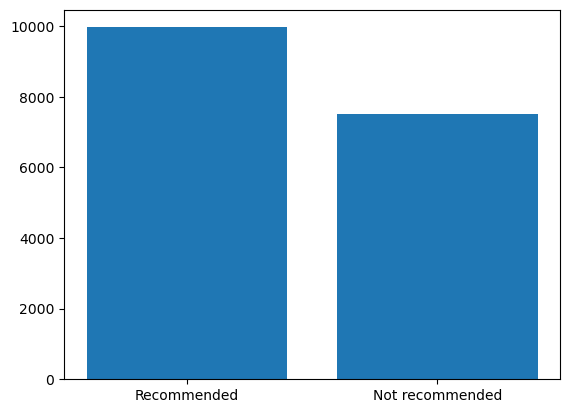
\includegraphics[scale=0.5]{plt1}
\end{figure}

\begin{figure}
\caption{'Data sample figure'}
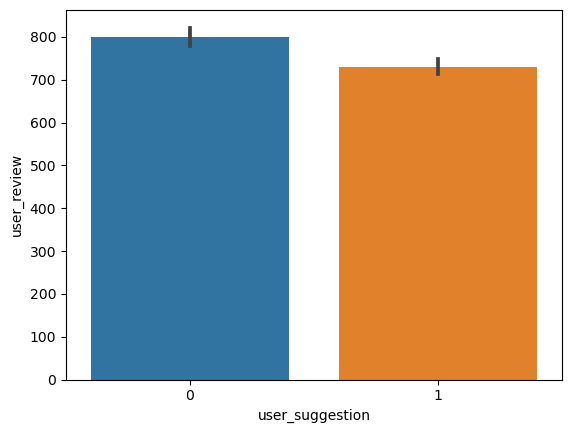
\includegraphics[scale=0.5]{plt2}
\end{figure}

\begin{figure}
\caption{'Results figure: what the sentiment analysis might look like on a successful
classifier'}
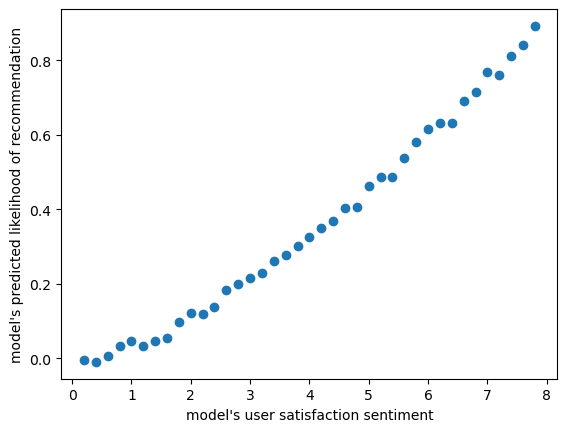
\includegraphics[scale=0.5]{plt3}
\end{figure}

\end{document}
